\documentclass[12pt,letterpaper]{article}
\usepackage{amsmath,amsthm,amsfonts,amssymb,amscd}
\usepackage{listings}
\usepackage{color}
\usepackage{MnSymbol,wasysym}
\usepackage{caption}
\usepackage{subcaption}
\definecolor{codegreen}{rgb}{0,0.6,0}
\definecolor{codegray}{rgb}{0.5,0.5,0.5}
\definecolor{codepurple}{rgb}{0.58,0,0.82}
\definecolor{backcolour}{rgb}{0.95,0.95,0.92}
\definecolor{dkgreen}{rgb}{0,0.6,0}
\definecolor{gray}{rgb}{0.5,0.5,0.5}
\definecolor{mauve}{rgb}{0.58,0,0.82}

\usepackage{biblatex}

\addbibresource{bibliography.bib}

\lstdefinestyle{mystyle}{
  language=R,
  backgroundcolor=\color{backcolour},   commentstyle=\color{codegreen},
  aboveskip=3mm,
  belowskip=3mm,
  showstringspaces=false,
  columns=flexible,
  basicstyle={\small\ttfamily},
  numbers=left,
  numbersep=5pt,
  numberstyle=\tiny\color{gray},
  keywordstyle=\color{blue},
  commentstyle=\color{dkgreen},
  stringstyle=\color{mauve},
  breaklines=true,
  breakatwhitespace=true
  tabsize=3
}

\lstset{style=mystyle}
\usepackage{hyperref}
\usepackage{graphicx}
\usepackage{enumerate}
\usepackage{fancyhdr}
\usepackage{mathrsfs}
\usepackage[margin=3cm]{geometry}
\setlength{\parindent}{0.0in}
\setlength{\parskip}{0.05in}

% Edit these as appropriate
\newcommand\course{CS432}
\newcommand\semester{Spring 2016}     
\newcommand\hwnum{5}
\newcommand\yourname{Kevin R. Clemmons}
\newcommand\login{oduprogrammer16}

\newenvironment{answer}[1]{
  \subsubsection*{Problem #1}
}

\pagestyle{fancyplain}
\headheight 40pt
\lhead{\yourname\ \\(\login)\\\course\ --- \semester}
\chead{\textbf{\Large Assignment \hwnum}}
\rhead{\today}
\headsep 40pt

\begin{document}

All files mentioned in this file are uploaded into the {\it github} repository.

The \LaTeX code invovled in the generation of this document was aided by the example code provided in the links that Dr. Nelson sent out on January 17, 2016\cite{mohammedaturban2013}. 

This document was compiled on \url{www.sharelatex.com}

\begin{answer}{1}
To determine whether or not the result of the split of the karate club could have been predicted, an R-Script called \textit{karateClubSimulation}, was created which implements the Girvan-Newman algorithm which was discussed in class\cite{michaelnelson}. The original code code for this implementation was found via the following url \url{https://github.com/maturban/cs595-f13/blob/master/assignment6/rcode.r}, modified to accept a datafile instead of retrieveing the data on the internet and the variables were renamed for clarification.  \\\\
%
The steps performed in the Girvan-Newman algorithm are as follows\cite{michaelnelson}:
\begin{enumerate}
    \item Calculate the edge betweeness for all the edges
    \item Determine the edge with the highest edge-betweeness. 
    \item Delete the edge with the highest edge-betweenness
    \item Repeat until the number of groups have been created from the initial graph. 
\end{enumerate} 

\newpage 
The code in Listing 1 shows the implementation of a single iteration of the Girvan-Newman algorithm. 
\begin{lstlisting}[language=R, caption=Single Iteration of Girvan-Newman Algorithm]
# Calculate betweeness of all edges 
edgeBetweeness <- edge.betweenness(karate_network)

# determine the highest edge betweeness 
highestEdgeBetweeness <- max(edgeBetweeness)

# Find the index with the highest edge betweeness
edgeToDelete <- match(c(highestEdgeBetweeness),edgeBetweeness)

# Delete the edge with the highest edgebetweeness 

# Get the start and end nodes
start <- get.edgelist(karate_network)[edgeToDelete,1] # The starting vertex
end <- get.edgelist(karate_network)[edgeToDelete,2]# The ending 

# Delete the edge with the highest edgebetweeness 
karate_network <- delete.edges(karate_network,E(karate_network,P=c(start,end)))
\end{lstlisting}

To draw the graph, igraph has a function which can determine groups or clusters of nodes as seen below in Listing 2\cite{rickyho2012,theigraphcoreteam}. 
%
\begin{lstlisting}[language=R,caption=Code for determining the number of clusters]
# Get the number of groups of nodes
numberOfClusters <- clusters(karate_network)['no']
\end{lstlisting}
%
The code in Listing 1 and Listing 2 exist inside a loop. The loop will terminate when the number in line 2 of Listing 2 is equal to two, indicating that two clusters of nodes have been created. Once an iteration is complete, a graph will be drawn depicting the current state of the graph using the code in Listing 3.\cite{theigraphcoreteam}.  \\\\ 
%
\begin{lstlisting}[language=R,caption=Code for Drawing the Current State of the Graph]
# Get list communities
communityList <- leading.eigenvector.community(karate_network,steps=1)

# Vertex Coloring
V(karate_network)$color <- ifelse(communityList$membership==1,"orange","yellow")

# Deterline scale of graph 
scale_graph <- function(vertex,alpha,beta){
	vertex <- vertex-min(vertex); vertex <-vertex/max(vertex); vertex <- vertex * (beta-alpha); vertex+alpha
}


E(karate_network)$color <- "grey"

# Plot the graph
tkplot(karate_network,layout=layout.kamada.kawai,vertex.label.font=2)

\end{lstlisting}

Once the algorithm is complete, a list all the edges in the order that they were deleted will be produced along with their computed edge-betweenness will be produced in a manner that can be copied and pasted into a table in \LaTeX . \\\\
The data that was used in the program, is written in a graph modeling format, models weighted graph of social interactions among friendship within a University in the United States during the 1970s \cite{waynewzachary1977,zachData}.  \\\\ 

The edges and the order in which they were deleted can be found in Table 1.
\begin{table}[ht!]
    \centering
    \begin{tabular}{|c|c|c|c|}\hline
    \textbf{Iteration Number} & \textbf{Starting Vertex} & \textbf{Ending Vertex} & \textbf{Edge-Betweeness} \\\hline
    1 & 1 & 32 & 71.3 \\\hline
    2 & 1  & 3 & 66.8 \\\hline
    3 & 1  & 9 & 77.3 \\\hline
    4 & 14 & 34 & 72.0 \\\hline
    5 & 20 & 34 & 123.2 \\\hline
    6 & 3 & 33 & 100.2 \\\hline
    7 & 2 & 31 & 143.6 \\\hline
    8 & 2 & 3 & 109.2 \\\hline
    9 & 3 & 4 & 107.6 \\\hline
    10 & 3 & 8 & 142.7 \\\hline
    11 & 3 & 14 & 285 \\\hline
    \end{tabular}
    \caption{Order of edges deleted during each iteration of the Girvan-Newman Algorithm}
    \label{tab:my_label}
\end{table}
\end{answer}


\newpage 
The following figures below visually depict each iteration of the Girvan-Newman algorithm. \\ 
\begin{figure}
\centering
\begin{subfigure}{.5\textwidth}
  \centering
  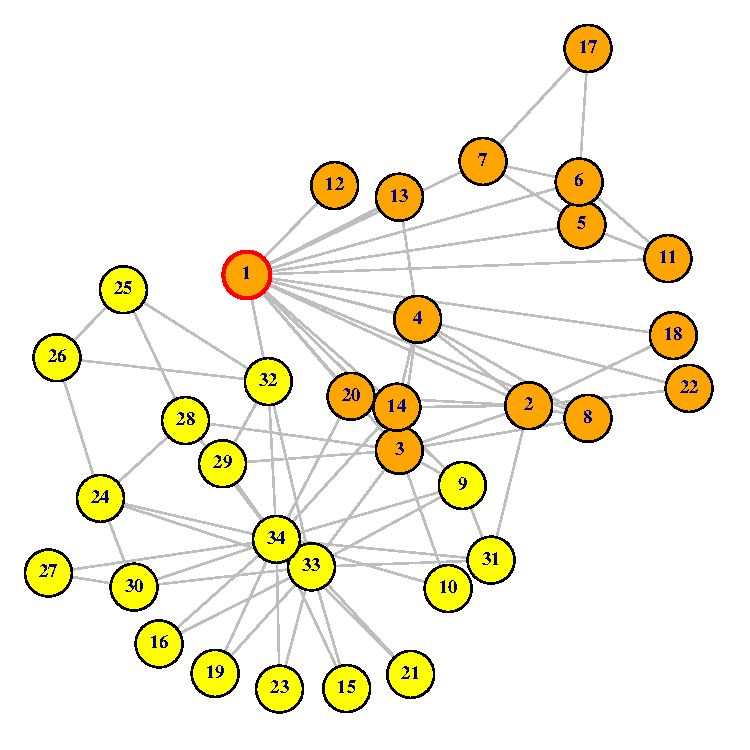
\includegraphics[width=.9\linewidth]{Plot1}
  \caption{Initial Graph}
  \label{fig:sub1}
\end{subfigure}%
\begin{subfigure}{.5\textwidth}
  \centering
  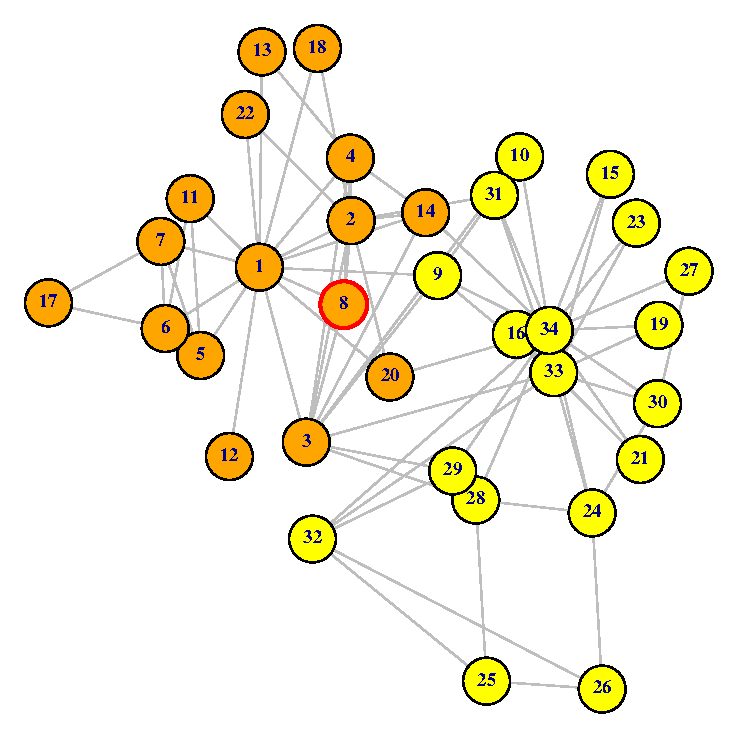
\includegraphics[width=.9\linewidth]{Plot2}
  \caption{After removing 1 $->$ 32}
  \label{fig:sub2}
\end{subfigure}
\caption{Inital Graph and Iteration 1}
\label{fig:test}
\end{figure}
%
\begin{figure}
\centering
\begin{subfigure}{.5\textwidth}
  \centering
  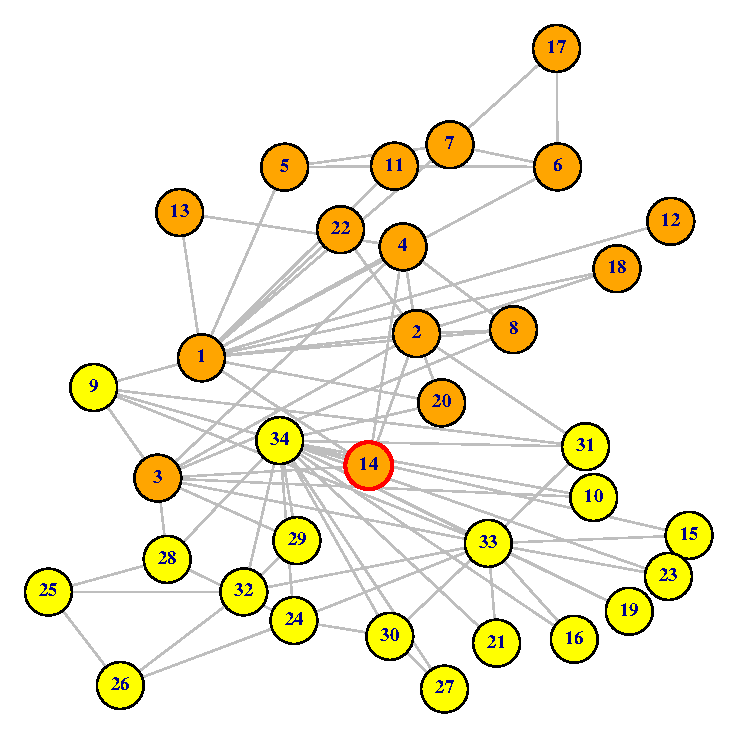
\includegraphics[width=.9\linewidth]{Plot3}
  \caption{After Removing 1 $->$ 3 }
  \label{fig:sub1}
\end{subfigure}%
\begin{subfigure}{.5\textwidth}
  \centering
  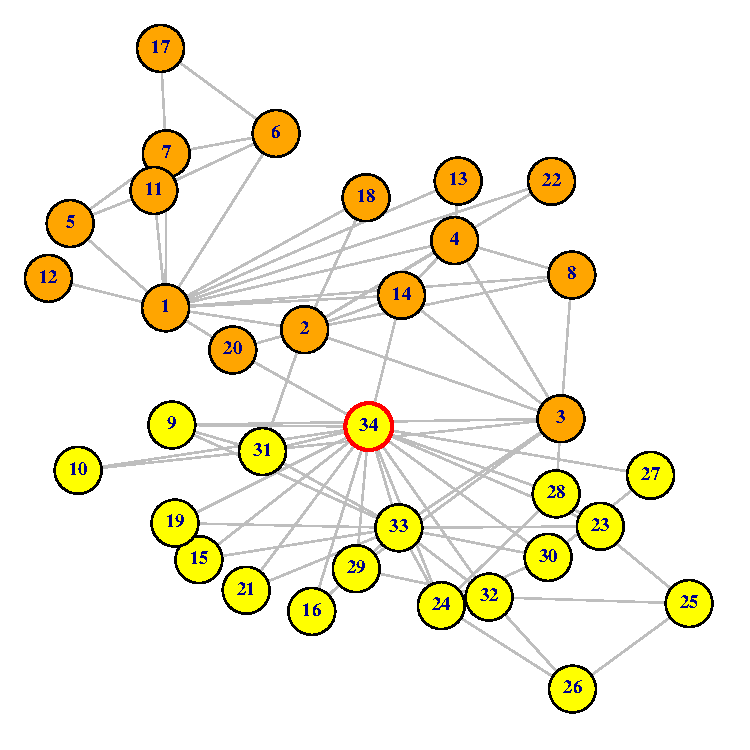
\includegraphics[width=.9\linewidth]{Plot4}
  \caption{After removing 1 $->$ 9}
  \label{fig:sub2}
\end{subfigure}
\caption{Iterations 2 and 3}
\label{fig:test}
\end{figure}
%
\begin{figure}
\centering
\begin{subfigure}{.5\textwidth}
  \centering
  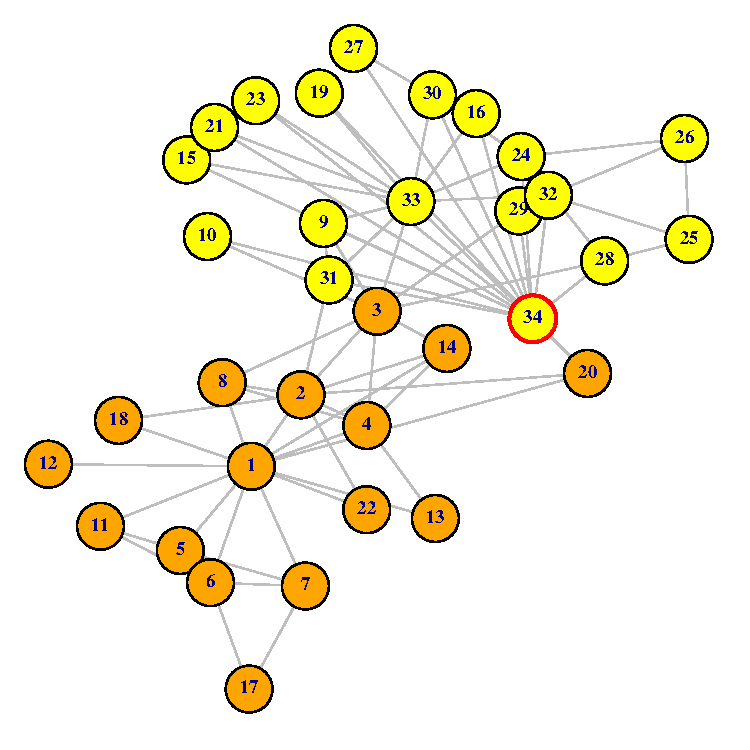
\includegraphics[width=.9\linewidth]{Plot5}
  \caption{After Removing 14 $->$ 34 }
  \label{fig:sub1}
\end{subfigure}%
\begin{subfigure}{.5\textwidth}
  \centering
  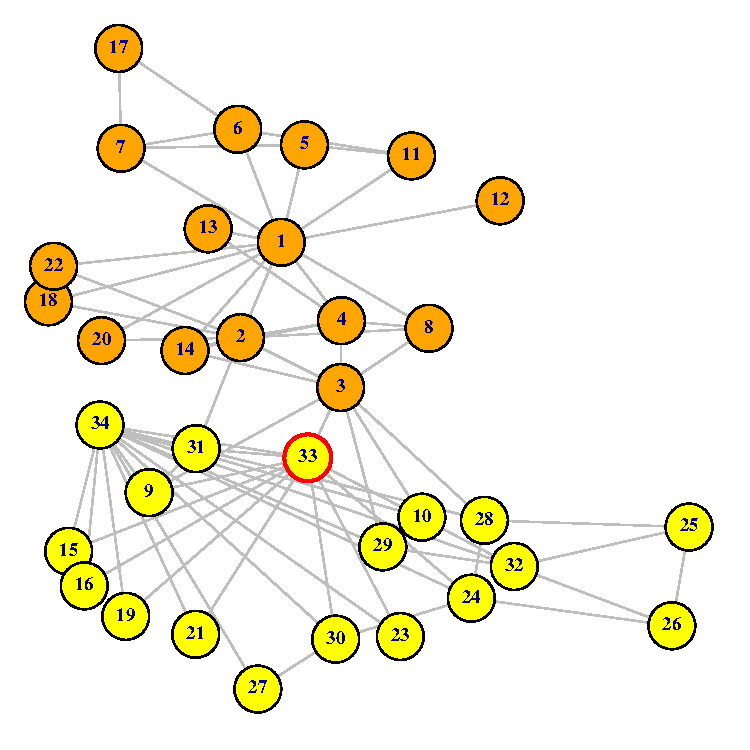
\includegraphics[width=.9\linewidth]{Plot6}
  \caption{After removing 20 $->$ 34}
  \label{fig:sub2}
\end{subfigure}
\caption{Iterations 4 and 5}
\label{fig:test}
\end{figure}
%
\begin{figure}
\centering
\begin{subfigure}{.5\textwidth}
  \centering
  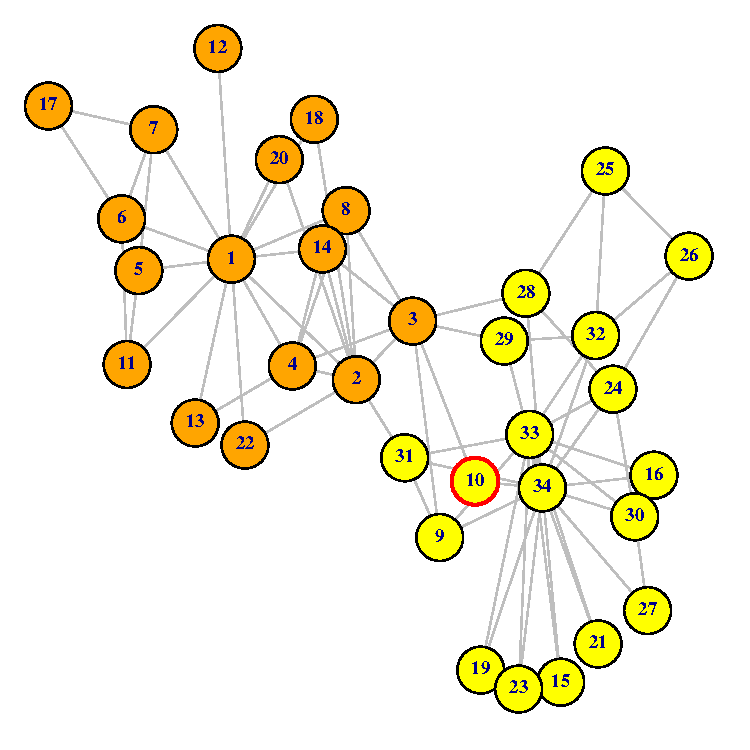
\includegraphics[width=.9\linewidth]{Plot7}
  \caption{After Removing 3 $->$ 33 }
  \label{fig:sub1}
\end{subfigure}%
\begin{subfigure}{.5\textwidth}
  \centering
  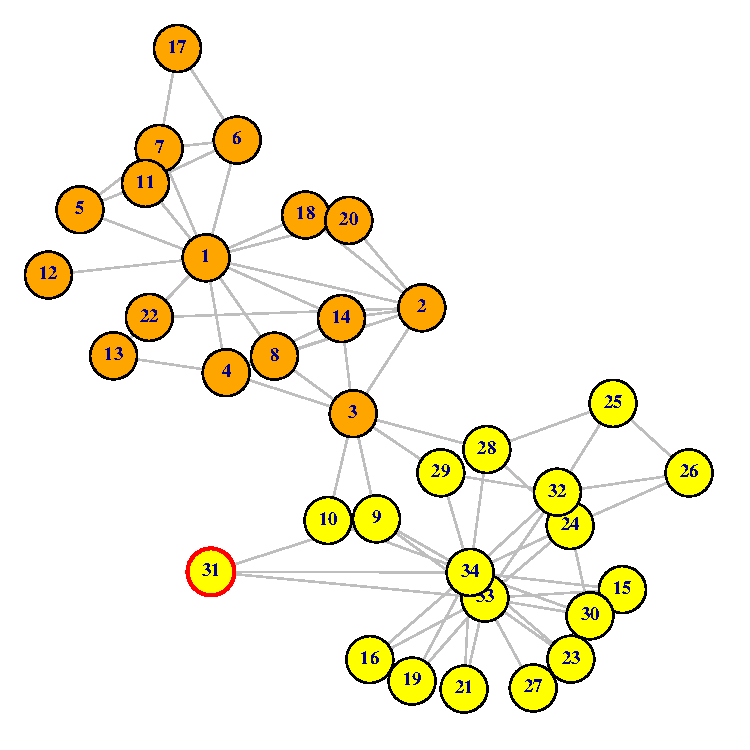
\includegraphics[width=.9\linewidth]{Plot8}
  \caption{After removing 2 $->$ 31}
  \label{fig:sub2}
\end{subfigure}
\caption{Iterations 6 and 7}
\label{fig:test}
\end{figure}
%
\begin{figure}
\centering
\begin{subfigure}{.5\textwidth}
  \centering
  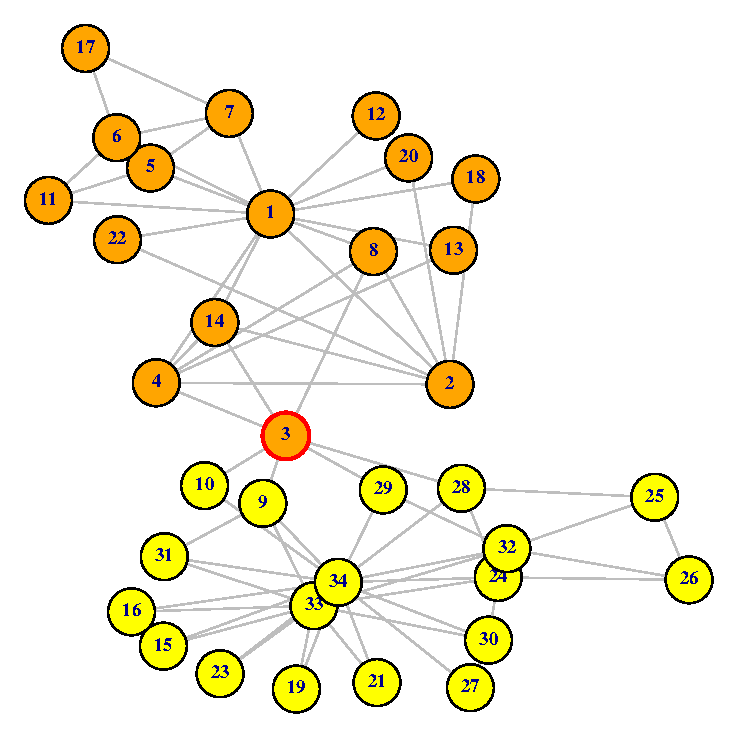
\includegraphics[width=.9\linewidth]{Plot9}
  \caption{After Removing 2 $->$ 3 }
  \label{fig:sub1}
\end{subfigure}%
\begin{subfigure}{.5\textwidth}
  \centering
  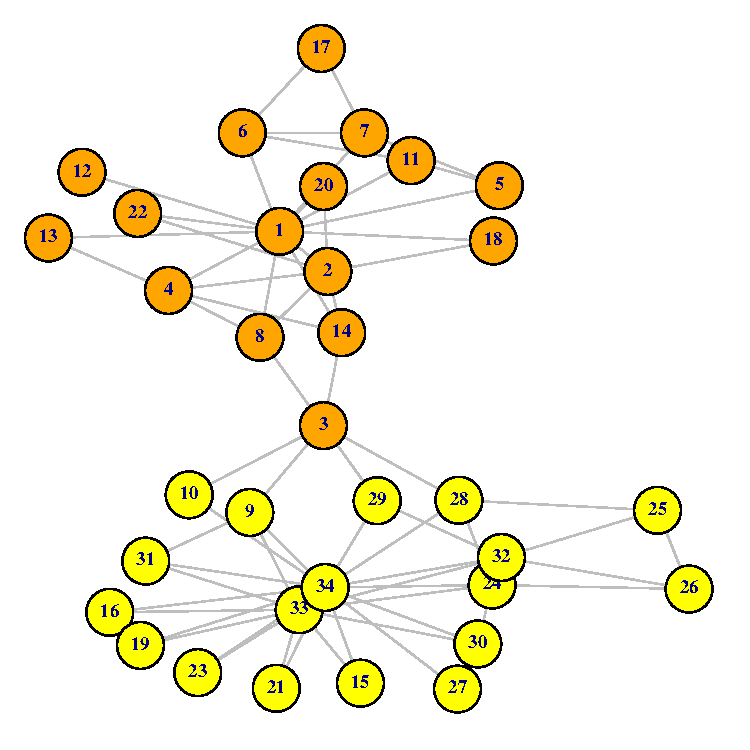
\includegraphics[width=.9\linewidth]{Plot10}
  \caption{After removing 3 $->$ 4}
  \label{fig:sub2}
\end{subfigure}
\caption{Iterations 8 and 9}
\label{fig:test}
\end{figure}
%
\begin{figure}
\centering
\begin{subfigure}{.5\textwidth}
  \centering
  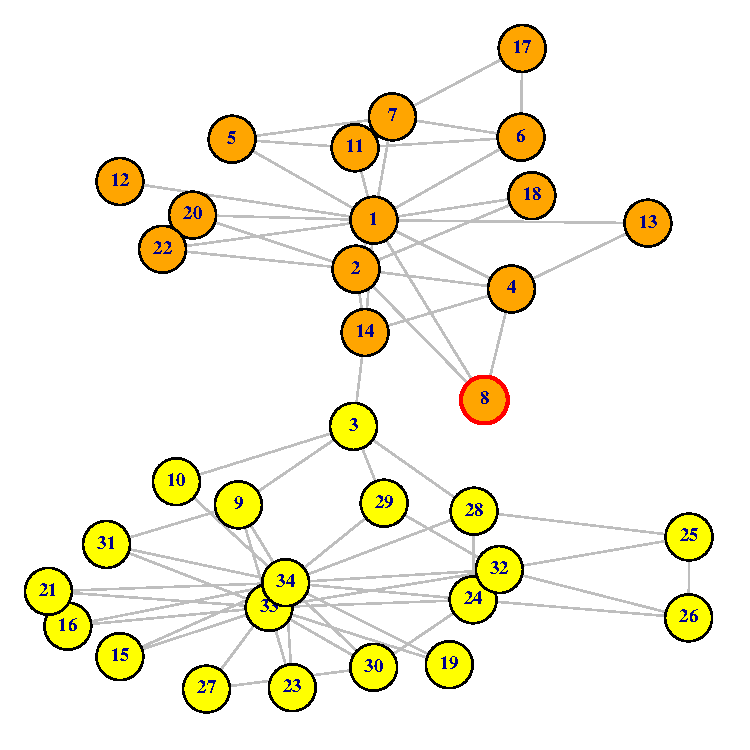
\includegraphics[width=.9\linewidth]{Plot11}
  \caption{After Removing 3 $->$ 8 }
  \label{fig:sub1}
\end{subfigure}%
\begin{subfigure}{.5\textwidth}
  \centering
  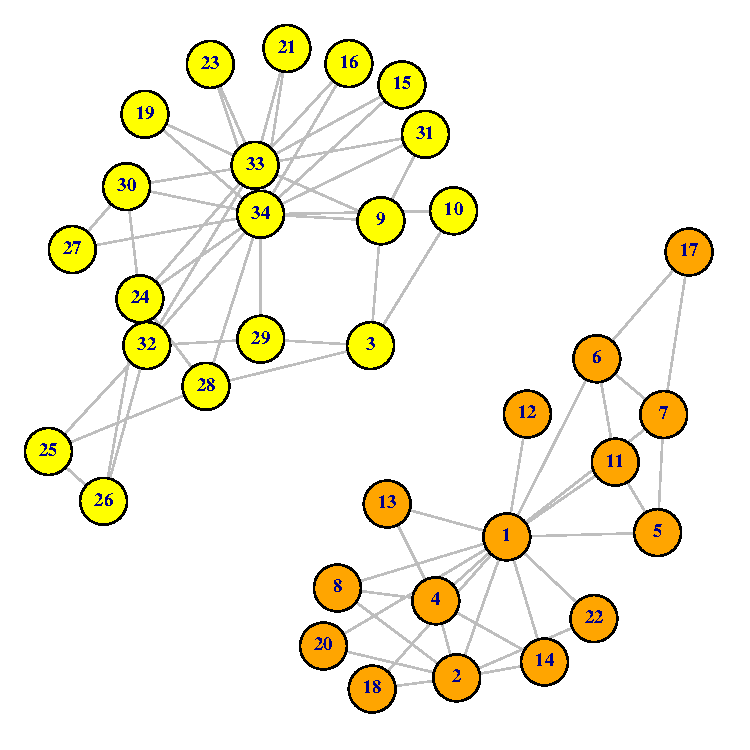
\includegraphics[width=.9\linewidth]{Plot12}
  \caption{After removing 3 $->$ 14}
  \label{fig:sub2}
\end{subfigure}
\caption{Iterations 10 and 11}
\label{fig:test}
\end{figure}


\newpage
Based on the graph obtained from running the program it is clearly evident that a weighted graph of social interactions can be used to predict the result of a split. It should be noted that in Figure 5-b and 6-a, that node 3 has switched groups. This indicates that the node may have changed it's mind to which group it belongs to or that perhaps maybe there exists limitation to how well the model can predict a split. 

\newpage 
\printbibliography

\end{document}
